\documentclass{standalone}
\usepackage{circuitikz,siunitx}
\usetikzlibrary{shadings,decorations.pathmorphing,arrows.meta,patterns}

\begin{document}
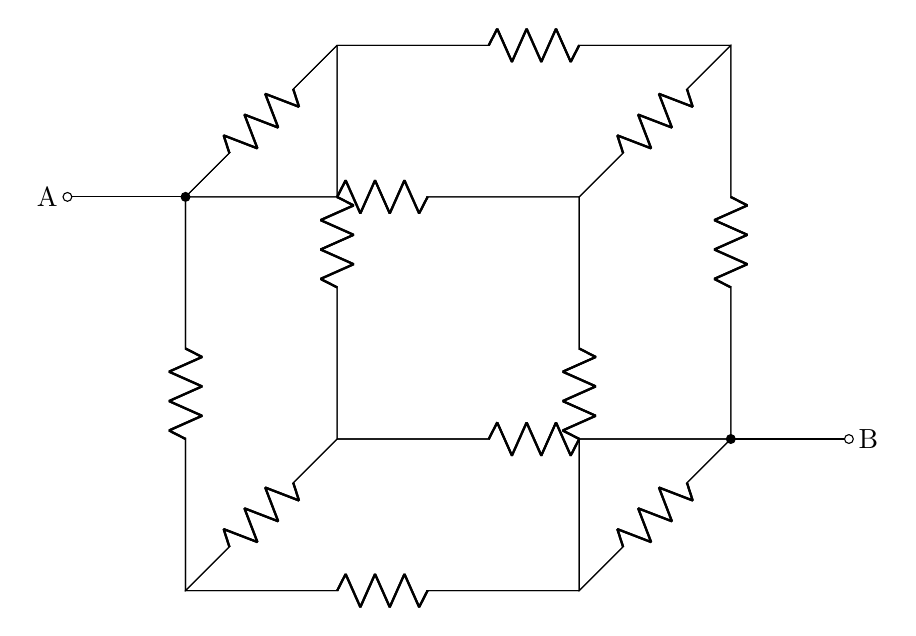
\begin{tikzpicture}
    \def\s{5}
    \coordinate (A) at (0,0,0);
    \coordinate (B) at (\s,0,0);
    \coordinate (C) at (\s,\s,0);
    \coordinate (D) at (0,\s,0);
    \coordinate (E) at (0,0,\s);
    \coordinate (F) at (\s,0,\s);
    \coordinate (G) at (\s,\s,\s);
    \coordinate (H) at (0,\s,\s);
    
    % Draw the cube
    \draw (A) to[R] (B) to[R] (C) to[R] (D) to[R] (A);
    \draw (A) to[R] (E) to[R] (F) to[R] (B) to[R] (A);
    \draw (B) to[R] (F) to[R] (G) to[R] (C) to[R] (B);
    \draw (C) to[R] (G) to[R] (H) to[R] (D) to[R] (C);
    \draw (D) to[R] (H) to[R] (E) to[R] (A) to[R] (D);
    \draw (E) to[R] (H) to[R] (G) to[R] (F) to[R] (E);
    \draw (H) to[short, *-o] ++(-1.5,0) node[left] {A};
    \draw (B) to[short, *-o] ++(1.5,0) node[right] {B};

    
\end{tikzpicture}
\end{document}